\documentclass{article}
    \usepackage{amssymb}
    \usepackage[utf8]{inputenc}
    \usepackage[russian]{babel}
    \usepackage[left=2cm,right=2cm,
        top=2cm,bottom=2cm,bindingoffset=0cm]{geometry}
    \usepackage{hyperref}
    \hypersetup{
        colorlinks=true,
        linkcolor=blue,
        filecolor=magenta,      
        urlcolor=cyan,
    }
  \usepackage{graphicx}
  \usepackage{booktabs}
  \usepackage{hyperref}
  \graphicspath{{pictures/}}
  \DeclareGraphicsExtensions{.pdf,.png,.jpg}
\usepackage{subcaption}
%\captionsetup{compatibility=false}

\begin{document}
\begin{center}{\hugeОтчет по дипломной работе за неделю\\}\end{center}
Дата: 1.4.2021\\
Научные руководители: Герасимов С.В., Мещеряков А.В.\\
Студент: Немешаева Алиса\\
Курс: 4\\

\renewcommand{\labelitemi}{$\blacksquare$}
\renewcommand\labelitemii{$\square$}
\begin{enumerate}
    \item Построен график ~\ref{Fig:N_src}{} для оценки количества детектированных скоплений в 
        зависимости от выбранного радиуса для поиска скоплений.\\
    \item Построен график ~\ref{Fig:Lambda} recall относительно параметров z и Lambda для 
        RedMaPPer. Параметр Lambda отвечает за <<богатство>> скопления, и от него зависит масса 
        скопления.\\
    \item Построена модель, продолжающая идею активного обучения. В этот раз в обучающую выборку 
        были добавлены те скопления, что были детектированы с $max\_pred \geqslant 0.8$. Результаты
        детекции на выбранной эпохе (20) на валидационной выборке представлены в таблице
        ~\ref{Tbl:Recall}.\\
\end{enumerate}




\begin{figure}[h]
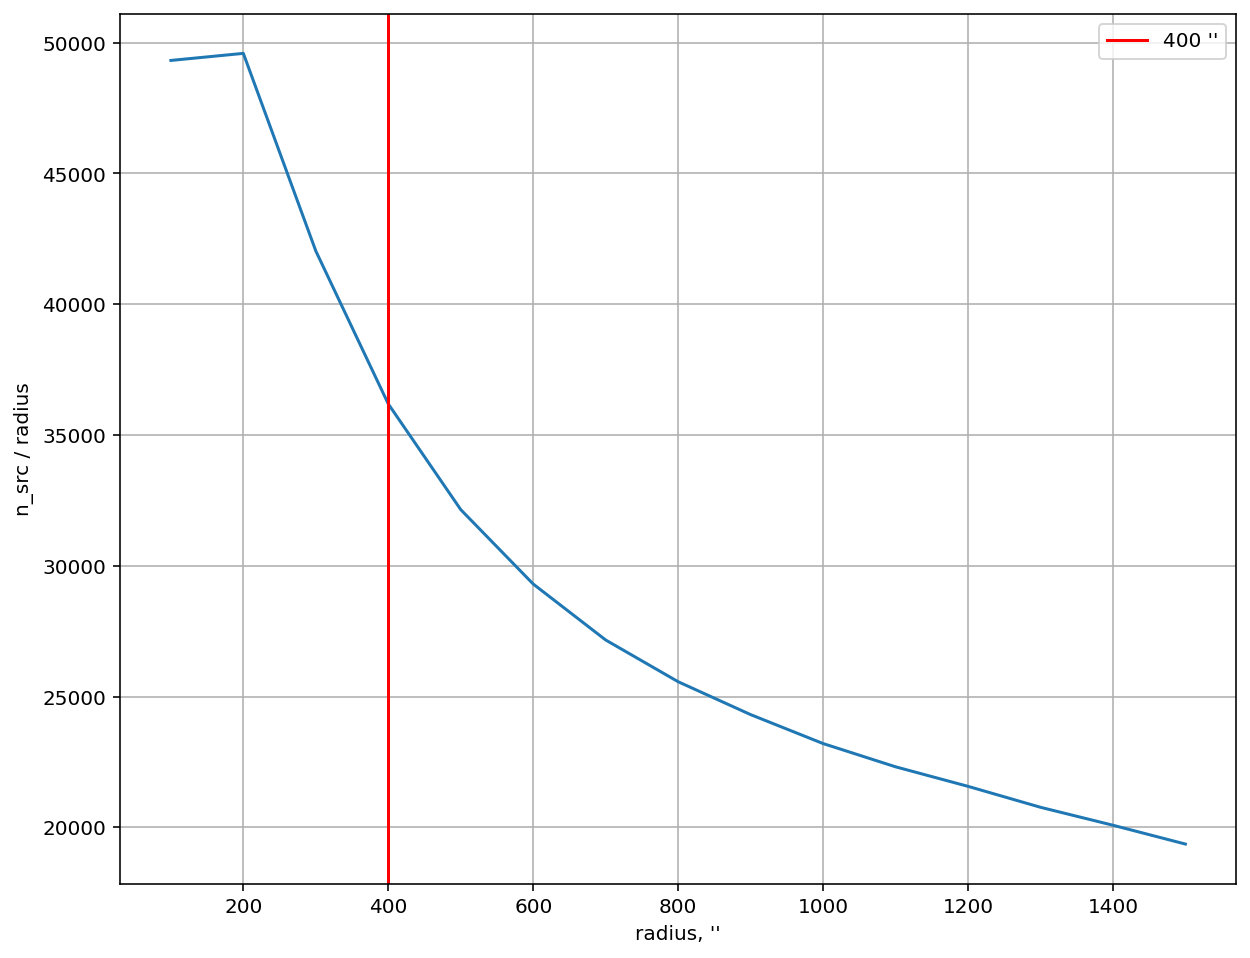
\includegraphics[width=0.8\linewidth]{n_src_rad}
\caption{График зависимости количества найденных скоплений от радиуса сопоставления.}
\label{Fig:N_src}
\end{figure}

\begin{figure}[h]
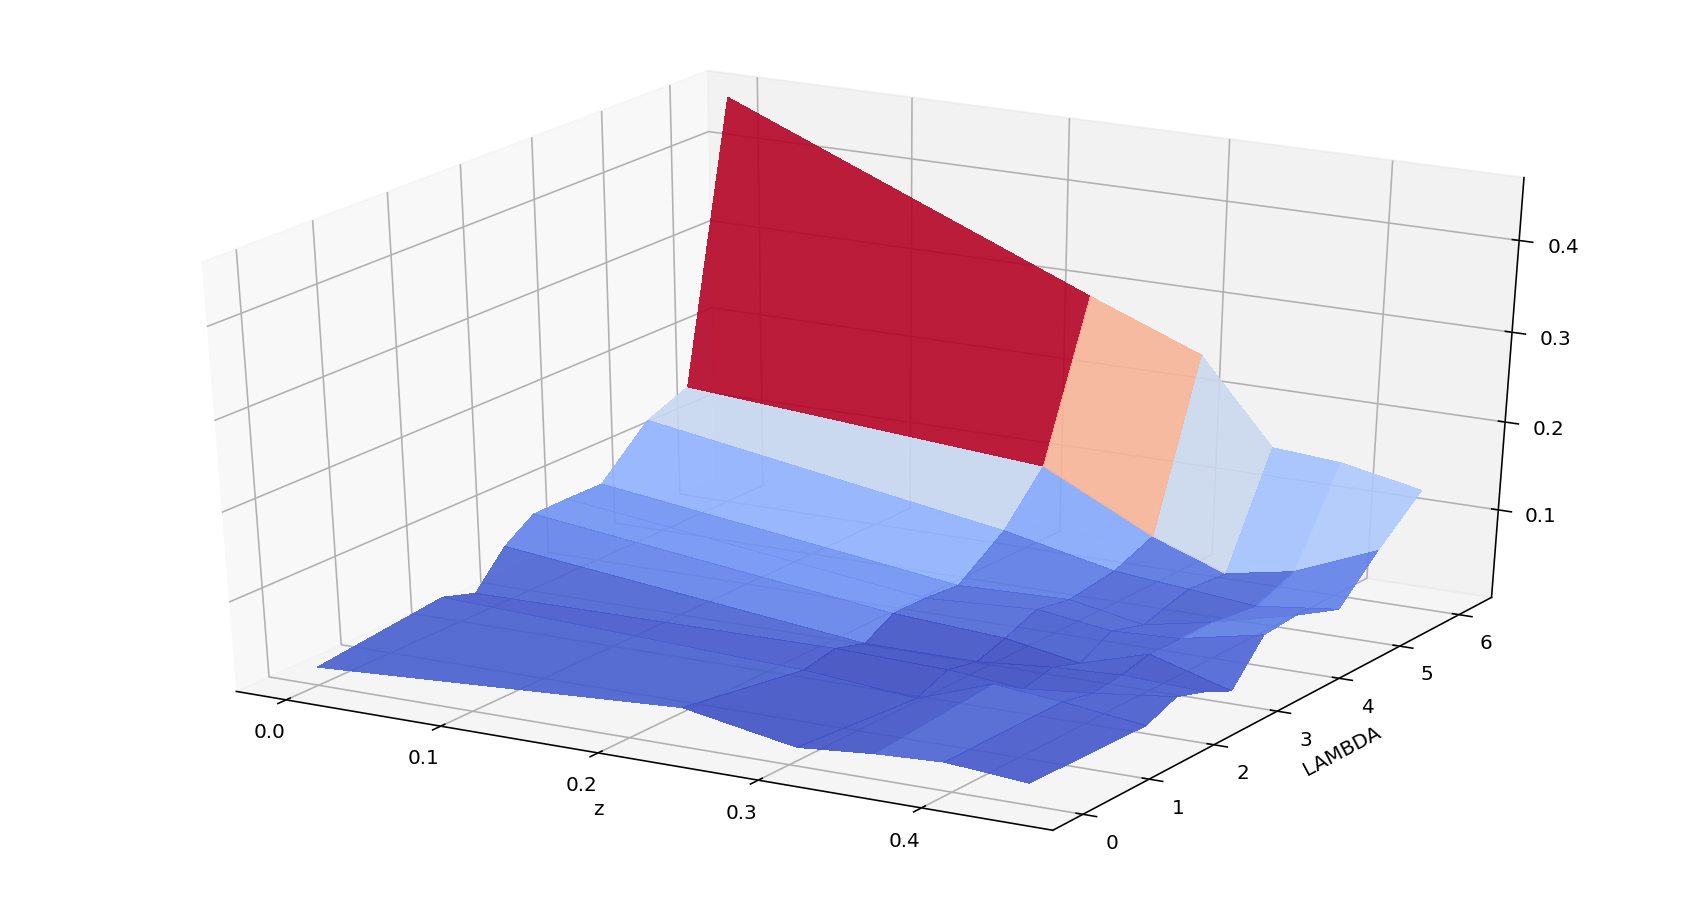
\includegraphics[width=0.8\linewidth]{lambda_3d}
\caption{График для сопоставления recall для каталога RedMaPPer относительно красного смещения z 
    и параметра Lambda.}
\label{Fig:Lambda}
\end{figure}

\begin{table}
\begin{tabular}{lrrrrrrr}
    \toprule
    {} &     PSZ2 &      MCXC &        RM &       ACT &     Abell &    fp &   all \\
    \midrule
    pz14                        &  0.93125 &  0.439759 &  0.043817 &  0.220930 &  0.213429 &   872 &  1181 \\
    pz\_rot28                    &  0.95000 &  0.463855 &  0.048685 &  0.225914 &  0.227818 &  1194 &  1531 \\
    pz\_act\_rot\_drop0.1\_ep9      &  0.91875 &  0.427711 &  0.037326 &  0.186047 &  0.196643 &   542 &   815 \\
    pz\_act\_feb\_rot\_drop0.3\_ep14 &  0.92500 &  0.427711 &  0.055826 &  0.235880 &  0.249400 &  1576 &  1938 \\
    pz\_act\_q\_0.1\_0.9\_14         &  0.94375 &  0.469880 &  0.048685 &  0.230897 &  0.225420 &  1201 &  1536 \\
    pz\_act\_found2\_22            &  0.93750 &  0.463855 &  0.053879 &  0.249169 &  0.235012 &  1145 &  1504 \\
    pz\_all\_found34              &  0.95000 &  0.481928 &  0.058423 &  0.244186 &  0.249400 &  1268 &  1644 \\
    pz\_all\_found2\_34            &  0.94375 &  0.493976 &  0.059072 &  0.244186 &  0.247002 &  1445 &  1821 \\
    pz\_found0.8\_20              &  0.93750 &  0.487952 &  0.056800 &  0.225914 &  0.235012 &  1230 &  1587 \\
\bottomrule
\end{tabular}
\caption{Таблица сравнения recall на основных моделях на валидационной выборке.}
\label{Tbl:Recall}
\end{table}

Отчет согласован с научным руководителем.\\
Общее количество строк кода за эту неделю: 260\\
\href{https://github.com/rt2122/data-segmentation-2}{Репозиторий}\\ 
\end{document}
